\documentclass[12pt, oneside]{article}
\usepackage{geometry}
\usepackage[utf8]{inputenc}
\usepackage{setspace}
\usepackage{times}
\usepackage{url}
\urlstyle{same}
\usepackage{multirow}
\usepackage[usegeometry]{typearea}
% Useful for checking layout
% \usepackage{showframe}
\usepackage{fancyhdr}
\usepackage{blindtext}
% Indenting the first sentence after section
\usepackage{indentfirst}
% Set language
\usepackage[german]{babel}
% Abbreviations
\usepackage{glossaries}
% For big tables which span multiple pages
\usepackage{longtable}
% Images
\usepackage{graphicx}
\graphicspath{ {./images/} }
% APA Citation Style
\usepackage[natbibapa]{apacite}
% Smaller font size for captions
\usepackage[font=small,labelfont=bf]{caption}

\geometry{
 a4paper,
 left=30mm,
 top=25mm,
 right=25mm,
 bottom=20mm,
 footskip=15pt,
}

\setstretch{1.3} % Define Line Spacing
\renewcommand{\headrulewidth}{0pt} % Remove footer line

\pagestyle{fancy} % Allow for customizing header and footer
% Customize footer for page number location
\fancyhf{}
\fancyfoot{}
\fancyhead[R]{Yannick Hutter}
\fancyhead[L]{Exposé}
\fancyfoot[R]{\thepage}



 \makeglossaries

 \newglossaryentry{dsr}
 {
     name=DSR,
     description={Design science Research}
 }
 \newglossaryentry{foph}
 {
     name=FOPH,
     description={Federal Office of Public Health}
 }
 \newglossaryentry{fhgr}
 {
     name=FHGR,
     description={Fachhochschule Graubünden}
 }
 \newglossaryentry{svi}
 {
     name=SVI,
     description={Social Vulnerability Index}
 }
 \newglossaryentry{who}
 {
     name=WHO,
     description={World Health Organisation}
 }



\begin{document}
\pagenumbering{roman}
\begin{titlepage}
	\begin{center}
		\Huge
		\textbf{Exposé}
		
		\vspace{0.5cm}
		\LARGE
		Analyse und Implementierung eines personalisierbaren Corona dashboards für Millenials
		
		\vspace{1.5cm}
		\normalsize
		\textbf{Yannick Hutter}\\
		\textbf{Digital Business Management Klasse 18tz}\\
		\textbf{Talackerstrasse 8}\\
		\textbf{8887 Mels}\\
		\textbf{yannick.hutter@stud.fhgr.ch}\\

		
		\vfill
		Referrent: Daniel Klinkhammer\\
		Korefferent: Michael Burch\\
		
		\vspace{0.8cm}
		
		
		Digital Business Management\\
		Fachhochschule Graubünden\\
		Mels, April 2022
	\end{center}
\end{titlepage}



\tableofcontents
\listoffigures
\listoftables
\printglossaries



\clearpage
\pagenumbering{arabic}
\setcounter{page}{2}

\section{Einleitung}
Die Coronavirus-Pandemie (fortlaufend als Corona bezeichnet) hat in grossen Teilen der Welt seine Spuren hinterlassen. So geht gemäss dem \Gls{foph} hervor, dass im Zeitraum vom 24.02.2020 bis zum 10.03.2022 mehr als 3 Millionen Ansteckungen in der Schweiz, sowie im Liechtenstein verzeichnet worden sind ~\citep{FOPH.13.03.2022}. Ein wichtiges Mittel zur Kommunikation mit der Bevölkerung sind hierbei Datenvisualisierungen, insbesondere Dashboards.
Der Begriff Dashboard kommt ursprünglich aus dem Englischen und bezieht sich auf das Armaturenbrett des Autos, wo alle relevanten Informationen übersichtlich auf einem Blick ersichtlich sind ~\citep{Duden.18.04.2022}.\\

Auch bei Corona wurde eine Vielzahl von Dashboard Visualisierungen erstellt, auf denen die wichtigsten Indikatoren der Pandemie wie Fallzahlen etc. ersichtlich sind. Ein Beispiel hierzu, welches versucht ein globales Bild wiederzugeben, ist das WHO Coronavirus Dashboard ~\citep{WHO.23.04.2022}. Auf diesem Dashboard sind Ansteckungszahlen, Todesfälle sowie Impfquoten ersichtlich. Das eine weltweite Organisation wie \Gls{who} sich um die Erstellung von Datenvisualisierungen zur Corona Thematik bemüht, soll aufzeigen, wie wichtig Dashboard-Visualisierungen und insbesondere Dashboards geworden sind.
\clearpage

\section{Forschungsfrage}
Die Landschaft der Corona Datenvisualisierungen ist sehr breit gestrickt und umfasst unterschiedlichste Repräsentanten von Visualisierungsarten. Nebst den einzelnen Visualisierungen wie Liniendiagramme, welche den zeitlichen Verlauf der Corona Ansteckungszahlen aufzeigen, werden diese aber auch in Form von Dashboards zusammengefasst. Eine grosse Anzahl dieser Dashboards sind jedoch sehr allgemein gehalten und zielen auf die breite Öffentlichkeit oder Datenanalysten als Zielgruppe ab. Auch lassen diese Dashboards sind sie einmal erstellt, keine Anpassungsmöglichkeiten durch den Nutzer selbst zu, sie sind nicht \textbf{personalisierbar}. Interessant in diesem Kontext ist es zu untersuchen, wie sich eine spezifische Nutzergruppe ein personalisierbares Corona Dashboard vorstellt und welche \textbf{Visualisierungsarten} von Relevanz sind. Aufgrund dieser explorativen Fragestellung ergibt sich folgende übergeordnete Forschungsfrage:


\begin{center}
\textbf{Wie stellen sich Millennials ein personalisierbares Corona Dashboard vor?}
\end{center}

Um diese Forschungsfrage abzudecken, wurden folgende untergeordnete Fragestellungen formuliert:

\begin{center}
\textbf{Welche Visualisierungstypen in Bezug auf Corona werden von FHGR Studierenden im Kontext eines personalisierbaren Corona Dashboards gefordert?\\
(untergeordnete Forschungsfrage 1)}
\end{center}

\begin{center}
\textbf{Welche Informationen in Bezug auf Corona werden von FHGR Studierende für ein Corona Dashboard gefordert?\\
(untergeordnete Forschungsfrage 2)}
\end{center}

\begin{center}
\textbf{Welche Personalisierungsmöglichkeiten werden von FHGR Studierende in Bezug auf Corona Dashboards gefordert?\\
(untergeordnete Forschungsfrage 3)}
\end{center}

\clearpage
\section{Methodische Vorgehensweise}
\subsection{Methodik}
Da es sich bei der übergeordneten Forschungsfrage um eine Fragestellung mit explorativem Charakter handelt, wird für die Methodik das Design Science Research (\Gls{dsr}) Modell nach Peffers verwendet (siehe Abbildung 1).


\begin{figure}[ht]
	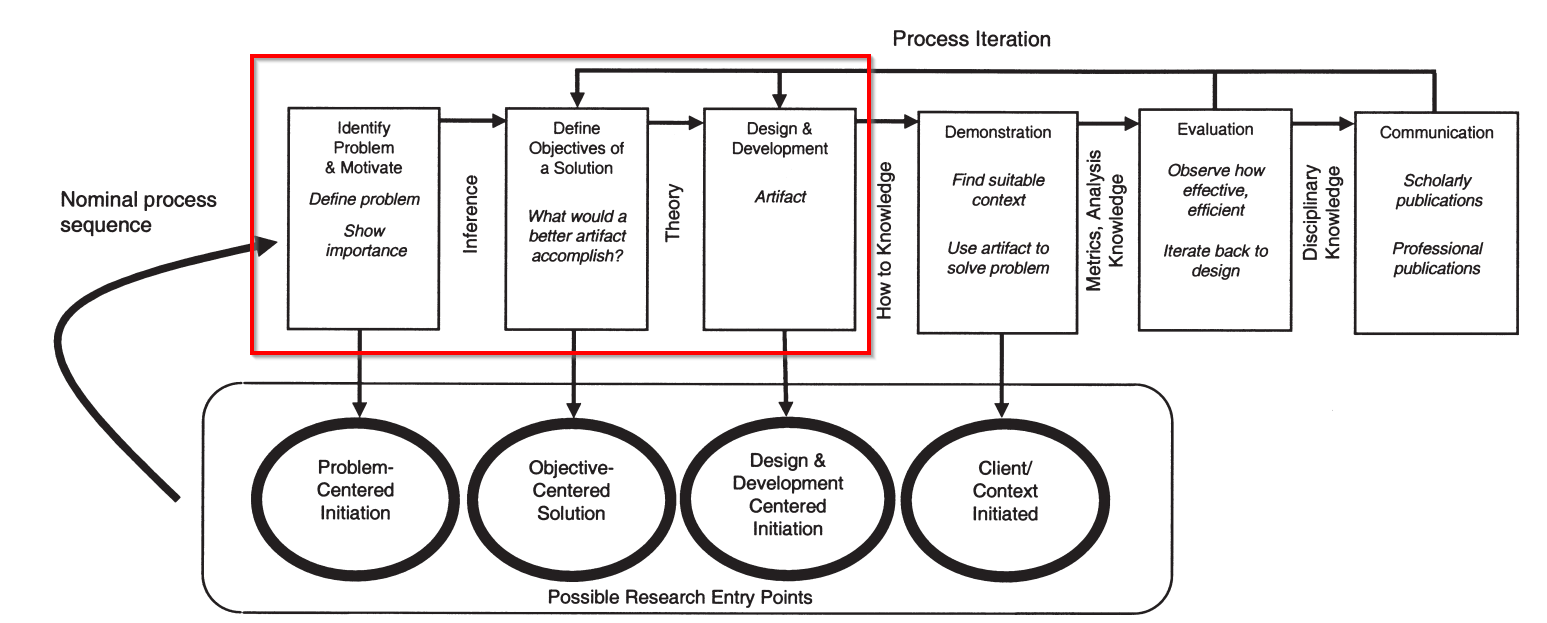
\includegraphics[width=12cm]{images/peffers_dsr_model.png}
	\centering
	\caption{DSR Modell nach Peffers ~\citep{K.Peffers.2007}}
\end{figure}

Bei diesem Modell gibt es mehrere Einstiegsmöglichkeiten (siehe \textit{Possible Research Entry Points}). Der Einstiegspunkt für die vorliegende Arbeit bildet der Punkt Problem-Centered Initiation. Das Problem, welches gelöst werden soll, ist die die starre Natur bestehender Corona Dashboards. Diese Dashboards lassen nach \textbf{der Erstellung für die angesprochene Zielgruppe} nicht mehr anpassen oder personalisieren. In diesem Kontext ist die Entwicklung eines Prototyps interessant, welcher die Erstellung der Dashboards \textbf{in die Hände der Zielgruppe selbst legt} und so auch personalisierungs- und Anpassungsmöglichkeiten bietet. Dies bildet somit bereits die Grundlage für den ersten Schritt des Models \textit{Identify Problem & Motivation}. Im zweiten Schritt \textit{Define Objective of a Solution} geht es darum, das Ziel einer möglichen Lösung aufzuzeigen. Anschliessend geht es im Schritt \textit{Design und Development} um die eigentliche Erstellung des Artefakts, was im Zuge dieser Arbeit ein High Fidelity Prototyp darstellt. Anschliessend würde es in den nächsten Schritten noch um die Evaluation des erstellten Prototyps, sowie die Publikation der Ergebnisse gehen. Jedoch ist das Ziel dieser Arbeit die Erstellung eines Prototyps aufgrund teilstrukturierter Interviews mit Millennials. Die eigentliche Evaluation des Prototyps kann im Rahmen einer weiterführenden Arbeit angegangen werden.

\clearpage
\subsection{Vorgehen}
Eine mögliche Art der Personalisierung von Dashboards besteht darin, von einem be-stehenden Katalog von Visualisierungen (Liniendiagramme welche Corona Fallzahlen darstellen etc.) seine gewünschten Favoriten auszuwählen und diese frei auf dem Dashboard zu platzieren. In einem ersten Schritt soll daher evaluiert werden, welche Corona Visualisierun-gen für Millennials von hoher Relevanz sind. Die Basis hierfür bildet die Studie von Zhang, welche eine Vielzahl von Corona Datenvisualisierungen untersuchte und die häufigsten Visualisierungsarten aus den verschiedenen Kategorien (Nachrichtentypen) analysierte ~\citep{YixuanZhang.}. In einem ersten Schritt werden Millennials dazu befragt, welche Visualisierungsart aufgrund des Nachrichtentyp Sie auf ihrem Corona Dashboard platzieren würden. Anschliessend wird Ihnen eine Auswahl von entsprechenden Visualisierungen aufgrund des zuvor gewählten Nachrichtentyps gezeigt, wovon Sie die passendste Visualisierung auswählen. Somit kann am Schluss ausgewertet werden, welche Visualisierung am relevantesten sind und die unter-geordnete Forschungsfrage I beantwortet werden. Eine entsprechende Auflistung mit den Nachrichtenkategorien und den dazugehörigen Visualisierungstypen kann dem Anhang entnommen werden (siehe Tabelle 2 im Anhang). Die entsprechenden Links zu den Visualisierungen können dem erstellten Codebook von Zhang entnommen werden ~\citep{YixuanZhang.2021}.\\

Um herauszufinden, welche Informationen Millennials in Zusammenhang mit Corona als relevant erachten, werden die Studierende aufgefordert 3 unterschiedliche Corona Dashboards zu besuchen und sich durch die entsprechende Navigation zu klicken. Währenddessen werden die Gedanken der Person mit Hilfe des thinking aloud Ansatzes festgehalten. Zum Schluss wird die Person über die relevantesten Informationen, welche Sie auf der Seite angetroffen hat, befragt (\textit{Welche Informationen waren für dich von besonderer Relevanz und warum?}). Somit kann mit Hilfe von bestehenden Corona Dashboards und dem thinking aloud Ansatz die untergeordnete Fragestellung 2 beantwortet werden.\\

Um den Personalisierungsaspekt in Bezug auf Dashboards zu untersuchen, wird eine Liste mit Personalisierungsmöglichkeiten gezeigt (Wählen von verschiedenen Themes, Anpassung von Schriftarten etc.). Anschliessend müssen von der Person entsprechende Favoriten gewählt werden. Somit kann die untergeordnete Fragestellung 3 mit Hilfe eines Rankings von bestehenden Optionen beantwortet werden.

\clearpage
\subsection{Aufbau}
Die Arbeit orientiert sich wie bereits erwähnt an den ersten drei Phasen des DSR Modells von Peffers. Demzufolge ergibt sich folgende Struktur:\\

\textbf{Einleitung}
\begin{itemize}
    \item Stand der Forschung
    \item Forschungsfrage
    \item Methodisches Vorgehen\\
\end{itemize}


\textbf{Problemidentifizierung und Motivation (Identify Problem und Motivation)}
\begin{itemize}
    \item Dashboard – Ein Begriff mit Ursprung in der Automobilindustrie
    \item Die wichtigsten Komponenten und Typen eines Dashboards
    \item Überblick über die bestehenden Corona Dashboards
    \item Motivation – Erstellung eines personalisierbaren Corona Dashboards für Millennials\\
\end{itemize}

\textbf{Identifikation der Ziele (Define Objectives of a Solution)}
\begin{itemize}
    \item Erstellung des Untersuchungsinstrumentes
    \item Evaluation von Visualisierungstypen für Corona Dashboards
    \item Identifikation von relevanten Informationen
    \item Identifikation von relevanten Personalisierungsmöglichkeiten in Bezug auf Dashboards\\
\end{itemize}

\textbf{Design und Development}
\begin{itemize}
    \item Design mittels Sketching
    \item High-Fidelity Prototyp als Web Applikation\\
\end{itemize}

\textbf{Reflexion und Limitationen}

\clearpage
\section{Stand der Forschung}
Die Coronavirus-Pandemie greift seit ihrem Aufkommen im Jahr 2019 in eine Vielzahl von Lebensbereichen ein. Es ist wenig verwunderlich, dass zu einem solch einschnei-dendem Thema eine grosse Anzahl von wissenschaftlichen Publikationen erstellt worden sind. Eine Publikation untersuchte die Vielzahl von Corona Datenvisualisierungen und weist ihnen verschiedene Arten von Intentionen (Aussage über den Verlauf der Pandemie etc.) zu ~\citep{YixuanZhang.}. Weitere Quellen untersuchten speziell für das Web zugeschnittene Corona Dashboards und leiteten daraus Design Guidelines ab ~\citep{Ivankovic.2021}. Andere Studien wiederum haben sich mit der Erstellung von Dashboards für spezielle Nutzergruppen auseinandergesetzt ~\citep{Ivanov.2018}. Auch wurde bereits im Zuge einer Studie die Schwierigkeiten bei der Erstellung von Corona Dashboards aus dem Blickwinkel der eigentlichen Ersteller evaluiert ~\citep{Barbazza.}. Jedoch scheint es zum jetzigen Zeitpunkt noch keine Studie zu geben, welche die Erstellung von \textbf{personalisierbaren} Corona Dashboards für eine bestimmte Zielgruppe behandelt unter Berücksichtigung eines Nutzerzentrierten Vorgehens untersucht.

\clearpage
\section*{Anhang}
\subsection*{Rechercheprotokoll}


\subsection*{Zeitplan}

\clearpage
\section*{Eigenständigkeitserklärung}
Hiermit bestätigt der Verfasser, dass die vorliegende Arbeit selbstständig verfasst und keine anderen als die angegebenen Hilfsmittel benutzt wurden. Stellen der Arbeit, die dem Wortlaut oder dem Sinn nach anderen Werken entnommen sind, wurden unter Angaben der Quelle kenntlich gemacht.

\begin{figure}[ht]
	
\includegraphics[width=6cm]{images/signature.png}
\end{figure}
Yannick Hutter, Mels am 01. Mai 2022

\clearpage
\bibliographystyle{apacite}
\urlstyle{rm}
\bibliography{main.bib}

\end{document}